\documentclass[11pt, a4paper]{article}
\usepackage[utf8]{inputenc}
\usepackage[T1]{fontenc}
\usepackage{polski}
\usepackage{graphicx}
\usepackage{float}
\usepackage{caption}
\usepackage{amsthm}
\usepackage{geometry}
\usepackage{longtable}
\usepackage{listings}
\usepackage{color}
\usepackage{subcaption}
\usepackage[section]{placeins}
\usepackage{fancyhdr}
\usepackage{graphicx}
\usepackage[polish]{babel}
\usepackage{dirtree}

\definecolor{dkgreen}{rgb}{0,0.6,0}
\definecolor{gray}{rgb}{0.5,0.5,0.5}
\definecolor{mauve}{rgb}{0.58,0,0.82}

\lstset{
  language=Java,
  aboveskip=3mm,
  belowskip=3mm,
  showstringspaces=false,
  columns=flexible,
  basicstyle={\small\ttfamily},
  numbers=none,
  numberstyle=\tiny\color{gray},
  keywordstyle=\color{blue},
  commentstyle=\color{dkgreen},
  stringstyle=\color{mauve},
  breaklines=true,
  breakatwhitespace=true,

}

\lstset{
  literate={ą}{{\k a}}1
  		     {Ą}{{\k A}}1
           {ż}{{\. z}}1
           {Ż}{{\. Z}}1
           {ź}{{\' z}}1
           {Ź}{{\' Z}}1
           {ć}{{\' c}}1
           {Ć}{{\' C}}1
           {ę}{{\k e}}1
           {Ę}{{\k E}}1
           {ó}{{\' o}}1
           {Ó}{{\' O}}1
           {ń}{{\' n}}1
           {Ń}{{\' N}}1
           {ś}{{\' s}}1
           {Ś}{{\' S}}1
           {ł}{{\l}}1
           {Ł}{{\L}}1
}

\geometry{
	a4paper,
	total={170mm,257mm},
	left=20mm,
	top=20mm,
}

\fancyhf{}
\fancyhead[L]{
\includegraphics[height=5.0mm]{PW.png}}

\fancyfoot{}
\renewcommand{\footrulewidth}{0.4pt}
\fancyfoot[C]{\thepage}

\setlength{\headheight}{6.50mm}
\pagestyle{fancy}

\title{\textbf{Uber Heals - specyfikacja funkcjonalna}\\
    Algorytmy i Struktury Danych}
\author{Paweł Cegielski, Piotr Szumański, Jakub Matłacz}
\date{data utworzenia: 3 grudnia 2020\\
    data ostatniej zmiany: 14 grudnia 2020}

\usepackage{natbib}
\usepackage{graphicx}

\begin{document}

\maketitle

\section{Wstęp}
Program udostępnia mapę obiektów, szpitali oraz dróg pomiędzy nimi. Pozwala wczytać listę pacjentów z pliku lub przy pomocy interfejsu graficznego. Wizualizuje transport tychże osób do najbliższych niepełnych szpitali. 

\section{Opis ogólny}
    \subsection{Nazwa programu}
    Nazwa programu to Uber Heals.
    \subsection{Poruszany problem}
    Problemem jest optymalna dystrybucja pacjentów, jednocześnie przestrzegając nałożonych ograniczeń takich jak istnienie dróg między lokacjami, ilość wolnych łóżek w szpitalach oraz położenie najbliższego szpitala od lokacji pacjenta.
    \subsection{Użytkownik docelowy}
    Program stworzono dla pracowników służby ochrony zdrowia odpowiedzialnych za transport pacjentów.
\section{Opis funkcjonalności}
    \subsection{Jak korzystać z programu?}
    Po uruchomieniu pliku .jar wyświetla się interfejs graficzny z pustą mapą oraz możliwością podania plików wejściowych: danych do naniesienia na mapę oraz listy pacjentów. Następnie można dane te wczytać najpierw tworząc mapę, a następnie, z zachowaniem kolejności, automatycznie dodawać kolejnych pacjentów. Ponadto użytkownik może dodać pacjenta na określonych współrzęnych z poziomu interfejsu. Można także zresetować pacjentów poprzez reset mapy.
    \subsection{Uruchomienie programu}
    Należy dwukrotnie kliknąć w plik .jar i czekać na otwarcie okna z GUI.
    \subsection{Możliwości programu}
    \begin{itemize}
        \item Wczytanie mapy z pliku.
        \item Wczytanie listy pacjentów z pliku.
        \item Stwierdzenie poprawności wczytanych danych.
        \item Stwierdzenie spójności i logiczności wczytanych danych.
        \item Wygenerowanie pliku z logami.
        \item Obliczenie dystrybucji pacjentów do szpitali.
        \item Wizualizacja dystrybucji pacjentów.
        \item Wyświetlanie intuicyjnych komunikatów błędów.
    \end{itemize}

\begin{figure}[ht]
    \centering
    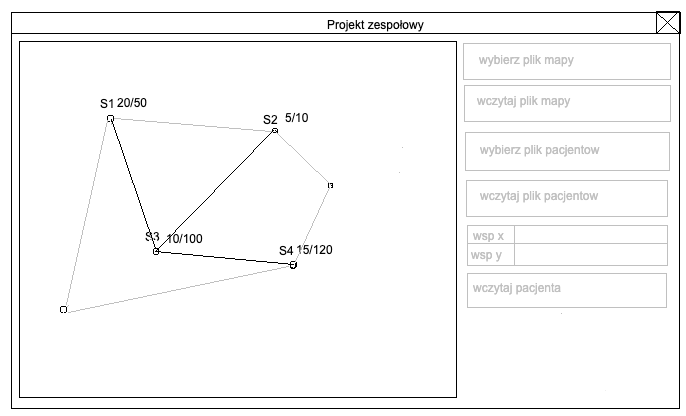
\includegraphics[width=1\textwidth]{okno.png}
    \caption{Schematyczny wygląd okna programu}
    \label{fig:folder}
\end{figure}
    
\section{Format danych i struktura plików}
    Pliki wejściowe powinny mieć rozszerzenie .txt. Logi programu mają to samo rozszerzenie co pliki wejściowe.
    \subsection{Struktura katalogów}
    Taka jak na Rysunku 2.
    \subsection{Dane wejściowe}
    \begin{itemize}
        \item Dane mapy
        \begin{lstlisting}
# Szpitale (id | nazwa | wsp. x | wsp. y | Liczba łóżek | Liczba wolnych łóżek)
1 | Szpital Wojewódzki nr 997 | 10 | 10 | 1000 | 100
2 | Krakowski Szpital Kliniczny | 100 | 120 | 999 | 99
3 | Pierwszy Szpital im. Prezesa RP | 120 | 130 | 99 | 0
4 | Drugi Szpital im. Naczelnika RP | 10 | 140 | 70 | 1
5 | Trzeci Szpital im. Króla RP | 140 | 10 | 996 | 0

# Obiekty (id | nazwa | wsp. x | wsp. y)
1 | Pomnik Wikipedii | -1 | 50
2 | Pomnik Fryderyka Chopina | 110 | 55
3 | Pomnik Anonimowego Przechodnia | 40 | 70

# Drogi (id | id_szpitala | id_szpitala | odległość)
1 | 1 | 2 | 700
2 | 1 | 4 | 550
3 | 1 | 5 | 800
4 | 2 | 3 | 300
5 | 2 | 4 | 550
6 | 3 | 5 | 600
7 | 4 | 5 | 750
\end{lstlisting}
        \item Dane pacjentów
        \begin{lstlisting}
# Pacjenci (id | wsp. x | wsp.y)
1 | 20 | 20
2 | 99 | 105
3 | 23 | 40
        \end{lstlisting}
    \end{itemize}

\begin{figure}[ht]
    \centering
    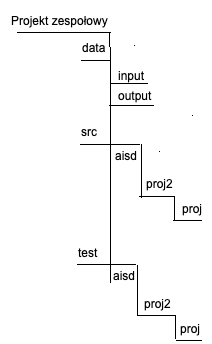
\includegraphics[width=0.3\textwidth]{katalogi.png}
    \caption{Struktura katalogów}
    \label{fig:folder}
\end{figure}

    \subsection{Dane wyjściowe}
    Dane wyjściowe będą przedstawiać wszystkie zdarzenia, zachodzące w procesie dystrybucji pacjentów, z zachowaniem kolejności. Ich przeznaczeniem jest umożliwienie odtworzenia ciągu zdarzeń w programie. 
\section{Scenariusz działania programu}
    \subsection{Scenariusz ogólny}
    \begin{enumerate}
        \item Uruchomienie pliku .jar.
        \item Pojawienie się okna z GUI.
        \item Wczytanie mapy z pliku.
        \item Wczytanie pacjentów z pliku lub ręcznie.
        \item Animacja dystrybucji pacjentów.
        \item Ewentualne zresetowanie mapy w trakcie.
        \item Zakończenie animacji.
        \item Zamknięcie okna aplikacji przez użytkownika.
    \end{enumerate}
    
\section{Środowisko}    
Do uruchomienia potrzebny jest system operacyjny Windows w wersji 10. Ponadto należy mieć zainstalowaną najnowszą Javę (wersja 8). 
\section{Testowanie}
Program podlegał testowaniu przy użyciu biblioteki JUnit 4.
\end{document}
